\documentclass[11pt,a4paper]{article}
\usepackage[T1]{fontenc}
\usepackage[utf8]{inputenc}
\usepackage[english]{babel}
\usepackage{amsmath,amssymb}
\usepackage[a4paper,margin=2cm]{geometry}
\usepackage{booktabs}
\usepackage{float}
\usepackage{graphicx}
\usepackage{hyperref}

\title{MLSF Project\\Meowdoku and SAT Solving}
\author{}
\date{October 2026}

% Lightweight numbered pseudocode (no external package needed).
\newcounter{pseudoline}
\newcounter{procedure}
\newcommand{\kw}[1]{\textbf{#1}}
\newcommand{\pinfo}[1]{\par\noindent\hspace*{2.4em}#1}
\newenvironment{pseudo}[2]
  {\par\medskip\noindent\begin{minipage}{\linewidth}\rule{\linewidth}{0.8pt}\par\noindent\refstepcounter{procedure}\label{#2}\textbf{Procedure~\theprocedure: #1}\par
   \noindent\rule{\linewidth}{0.4pt}\setcounter{pseudoline}{0}\small}
  {\par\noindent\rule{\linewidth}{0.8pt}\end{minipage}\par\medskip}
\newcommand{\pline}[2]{\par\stepcounter{pseudoline}\noindent
  \hbox to 1.8em{\hfil\scriptsize\thepseudoline\hspace{0.6em}}%
  \hspace*{\dimexpr 1.4em*#1\relax}%
  \parbox[t]{\dimexpr\linewidth-1.8em-1.4em*#1\relax}{#2}}

\begin{document}
\maketitle

\section*{Project overview}

The project builds a SAT solver and uses it to solve Meowdoku. In a Meowdoku grid, each cell belongs to one colored region. Cats must be placed so that each region contains exactly one cat, each row and column contains at most one cat, and no two cats touch, including diagonally. A SAT problem asks whether there is an assignment of true or false to Boolean variables that makes a formula true. By assigning one variable to each cell, the game rules can be written as a formula whose satisfying assignments correspond to legal cat placements.

The work forms a sequence. First, a grid is converted into clauses in DIMACS CNF format, the standard text representation used here for SAT instances. Next, a DPLL solver reads those clauses and searches for a satisfying assignment. A satisfying assignment can then be translated back into cat coordinates and displayed on the original grid. Later questions change how the solver chooses its search branches, measure the effects, and specify the final command-line interface. Each stage uses the output of the preceding stage.

\begin{enumerate}
\item \textbf{\hyperref[sec:q1]{Question 1 --- Model and generate grids.}} Define the Boolean variable for each cell; express the four game rules as CNF clauses; write a converter from the required grid format to DIMACS; and generate grids that have at least one solution by construction.
\item \textbf{\hyperref[sec:q2]{Question 2 --- Read and solve CNF.}} Parse DIMACS into a Python formula, implement the status-only and model-producing versions of DPLL, validate them on the supplied instances, and discuss their performance.
\item \textbf{\hyperref[sec:q3]{Question 3 --- Present a game solution.}} Connect the grid converter to the SAT solver. Convert a satisfying assignment back into cell coordinates, write the required region-by-region and marked-grid output, and check that the placement obeys the game rules.
\item \textbf{\hyperref[sec:q4]{Question 4 --- Improve branch selection.}} Implement and compare at least four DPLL branching heuristics. The selection must include a literal-based rule, a rule that uses clause sizes, and a dynamic rule based on the current simplified formula.
\item \textbf{\hyperref[sec:q5]{Question 5 --- Measure the heuristics.}} Instrument the solvers, compare their search effort and run time on varied SAT and UNSAT instances, and analyze whether the extra work of choosing branches pays off.
\item \textbf{\hyperref[sec:q6]{Question 6 --- Provide the final solver interface.}} Offer both the basic \texttt{dpll} mode and an \texttt{optimized} mode through \texttt{sat.py}, using the prescribed SAT/UNSAT and optional model output format.
\end{enumerate}

\section{Question 1: Encoding and generating Meowdoku grids}\label{sec:q1}

\begin{center}
\begin{tabular}{@{}p{6.2cm}p{10cm}@{}}
\toprule
File & Description\\
\midrule
\texttt{image\_grid.txt} & The board of Figure~\ref{fig:meowdoku-board} in the grid-file format of the assignment (\texttt{GRID}, \texttt{ZONES}, then one line of region labels per row). Input of the converter.\\
\texttt{meowdoku\_to\_dimacs.py} & Converter from a grid file to a DIMACS CNF file: \texttt{read\_grid}, \texttt{encode\_grid} and \texttt{write\_dimacs}.\\
\texttt{generate\_grid.py} & Generator of square boards with a planted solution: \texttt{cat\_columns} plants the cats, \texttt{generate\_grid} grows the regions, and \texttt{write\_grid} writes the grid file.\\
\bottomrule
\end{tabular}
\end{center}

\subsection{The board and its variables}

A Meowdoku grid has $N$ rows, $M$ columns, and $K$ disjoint colored regions. A legal placement has at most one cat in each row and column, exactly one cat in each region, and no two cats in cells that touch along an edge or corner. Figure~\ref{fig:meowdoku-board} is the single running example in this report; ``the board'' below always refers to it. It has $N=M=K=6$, and its six cats show a complete legal placement. The SAT input uses the colored regions; the cats of Figure~\ref{fig:meowdoku-board} illustrate a solution rather than fixed clues in the input file.

\begin{figure}[htbp]
\centering
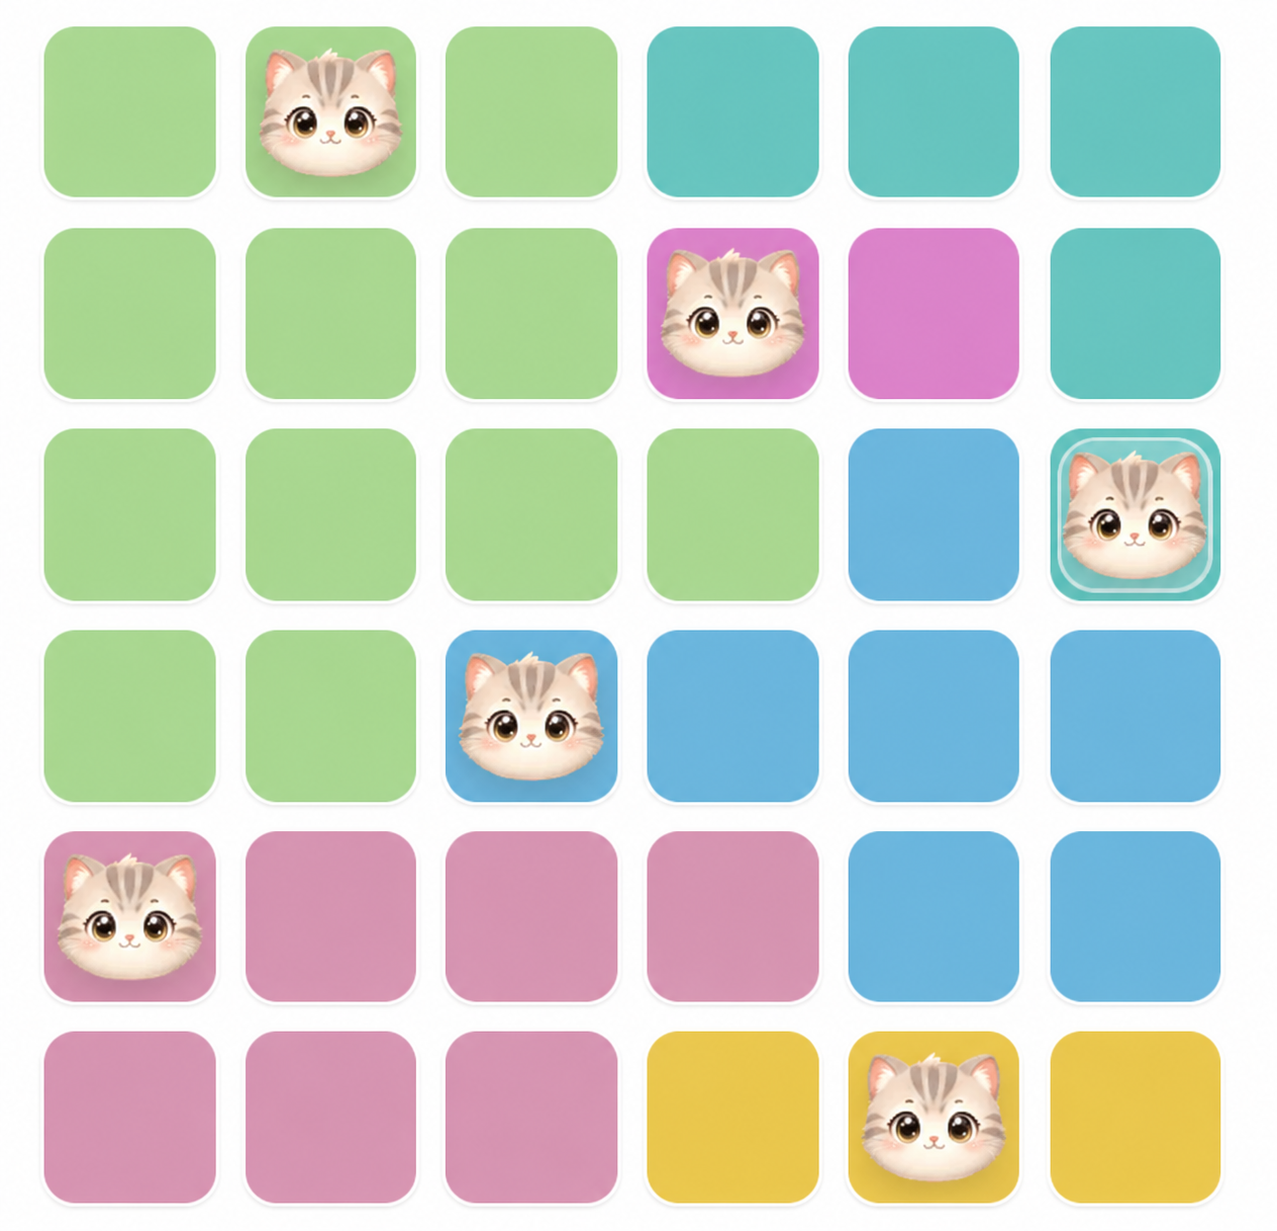
\includegraphics[width=0.55\linewidth]{figures/meowdoku_board.png}
\caption{Example of a $6\times6$ Meowdoku board. Colors define the six regions, and the six cats show a complete solution.}
\label{fig:meowdoku-board}
\end{figure}

We name the green, turquoise, pink, blue, mauve, and yellow regions A, B, C, D, E, and F, respectively. The colors give the following complete grid description, saved as \texttt{image\_grid.txt}:
\begin{verbatim}
GRID 6 6
ZONES A B C D E F

A A A B B B
A A A C C B
A A A A D B
A A D D D D
E E E E D D
E E E F F F
\end{verbatim}
Each of the six final lines describes one row, from top to bottom; each label identifies the region of one cell, from left to right. Thus the pink region is $R_C=\{(2,4),(2,5)\}$, whereas the green region includes cells in four different rows. The file records regions, not cat positions. Let $R_A,\ldots,R_F$ denote the sets of cells carrying the corresponding labels. These six nonempty sets partition all 36 cells. In formulas indexed by $r=1,\ldots,K$, we identify $R_1=R_A,\ldots,R_6=R_F$.

For every cell $(i,j)$, with row $i$ and column $j$ numbered from 1, introduce a Boolean variable $x_{i,j}$. It is true exactly when a cat is in that cell. A negative literal $\neg x_{i,j}$ means that the cell is empty. DIMACS represents each variable with an integer:
\[
\operatorname{id}(i,j)=(i-1)M+j=(i-1)6+j.
\]
The first term skips the $i-1$ preceding rows of six cells; adding $j$ selects the cell in row $i$. For example, the cat in pink cell $(2,4)$ corresponds to $\operatorname{id}(2,4)=(2-1)6+4=10$, so its variable is $x_{2,4}$ and its DIMACS positive literal is \texttt{10}. The yellow cat in $(6,5)$ has variable number $(6-1)6+5=35$. All 36 cells have distinct IDs from 1 to 36:
\[
\begin{array}{c|rrrrrr}
 & j=1&j=2&j=3&j=4&j=5&j=6\\ \hline
 i=1&1&2&3&4&5&6\\
 i=2&7&8&9&10&11&12\\
 i=3&13&14&15&16&17&18\\
 i=4&19&20&21&22&23&24\\
 i=5&25&26&27&28&29&30\\
 i=6&31&32&33&34&35&36
\end{array}.
\]

The following table lists every variable belonging to each region. It is equivalent to the colored grid because the preceding formula converts every listed ID back to a unique cell.
\begin{center}
\begin{tabular}{@{}lp{9cm}r@{}}
\toprule
Region & Cell-variable IDs & $s_r=|R_r|$\\
\midrule
A (green) & 1, 2, 3, 7, 8, 9, 13, 14, 15, 16, 19, 20 & 12\\
B (turquoise) & 4, 5, 6, 12, 18 & 5\\
C (pink) & 10, 11 & 2\\
D (blue) & 17, 21, 22, 23, 24, 29, 30 & 7\\
E (mauve) & 25, 26, 27, 28, 31, 32, 33 & 7\\
F (yellow) & 34, 35, 36 & 3\\
\bottomrule
\end{tabular}
\end{center}

The six cats in Figure~\ref{fig:meowdoku-board} occupy $(1,2)$, $(2,4)$, $(3,6)$, $(4,3)$, $(5,1)$, and $(6,5)$, with IDs $2$, $10$, $18$, $21$, $25$, and $35$. The corresponding satisfying assignment sets exactly
\[
T=\{x_{1,2},x_{2,4},x_{3,6},x_{4,3},x_{5,1},x_{6,5}\}
\]
to true and all other cell variables to false. The six cats occupy different rows, columns, and regions. Their column sequence $2,4,6,3,1,5$ has gaps greater than one between consecutive rows, so none touch diagonally.

\subsection{From an expression to DIMACS}

A \emph{literal} is a variable or its negation. Literals joined by $\lor$ (OR) form a \emph{clause}; clauses joined by $\land$ (AND) form a formula in \emph{conjunctive normal form} (CNF). Every clause must be true. The symbols $\bigvee$ and $\bigwedge$ repeat OR and AND over the indices written below them. A comma in an index lists simultaneous conditions; it is not itself a logical operator.

The pink region has only the cells $(2,4)$ and $(2,5)$. Requiring exactly one cat there gives the small CNF fragment
\[
\underbrace{(x_{2,4}\lor x_{2,5})}_{\text{at least one}}
\land
\underbrace{(\neg x_{2,4}\lor\neg x_{2,5})}_{\text{at most one}}.
\]
Their IDs are 10 and 11. As a standalone two-clause fragment using the board's 36 variable numbers, the expression becomes
\begin{verbatim}
p cnf 36 2
10 11 0
-10 -11 0
\end{verbatim}
In general, the DIMACS header has the form \texttt{p cnf V C}: $V$ is the number of Boolean \emph{variables}, and $C$ is the number of clauses that follow. There is one variable per cell, so the board has $V=NM=6\cdot6=36$. The two clauses above are only a fragment of the complete formula, hence $C=2$ in this example. Each OR-clause becomes one line, and placing both lines in the file represents AND. A positive number denotes a variable and a negative number its negation. Zero ends a clause; it is a delimiter, not variable zero or the Boolean value false.

The complete board formula contains additional clauses for all four rules, each written in the same DIMACS format.

\subsection{The four rules as clauses}

\subsubsection{At most one cat in each row}

For distinct cells $(i,j)$ and $(i,k)$ in the same row, at least one must be empty. The clause $\neg x_{i,j}\lor\neg x_{i,k}$ is false precisely when both contain cats. We write it for every pair of columns $j<k$ in every row $i$:
\[
F_{\mathrm{rows}}=
\bigwedge_{1\le i\le N,\;1\le j<k\le M}
\underbrace{(\neg x_{i,j}\lor\neg x_{i,k})}_{\text{not both cats in row }i}.
\]
For example, in the first row, cells $(1,2)$ and $(1,3)$ have IDs 2 and 3. Their clause becomes \texttt{-2 -3 0}. The cat at $(1,2)$ makes $x_{1,2}$ true, so the clause requires $x_{1,3}$ to be false. We need a clause for every pair, since excluding only this pair would still allow cats at other two cells of the row. The condition $j<k$ visits each unordered pair once and never pairs a cell with itself. These clauses allow zero or one cat in a row, exactly as the rule states.

\subsubsection{At most one cat in each column}

Two cells in one column have the same $j$ and different row numbers $i<k$. Applying the same pairwise exclusion gives
\[
F_{\mathrm{columns}}=
\bigwedge_{1\le j\le M,\;1\le i<k\le N}
\underbrace{(\neg x_{i,j}\lor\neg x_{k,j})}_{\text{not both cats in column }j}.
\]
In column 4, the cat at $(2,4)$ has ID 10, while yellow cell $(6,4)$ has ID 34. The clause $\neg x_{2,4}\lor\neg x_{6,4}$ becomes \texttt{-10 -34 0}. Since the cat at $(2,4)$ makes the first literal false, $(6,4)$ must remain empty. The rule covers any two cells in a column, even if they are not adjacent.

\subsubsection{Exactly one cat in each region}

For a region $R_r$, one positive clause requires at least one cat. Negative clauses for all pairs of distinct cells prevent a second cat. Both conditions must hold for every region:
\[
F_{\mathrm{regions}}=
\bigwedge_{1\le r\le K}
\left[
\underbrace{\left(\bigvee_{u\in R_r}x_u\right)}_{\text{at least one cat}}
\land
\underbrace{\left(\bigwedge_{\{u,v\}\in\binom{R_r}{2}}
(\neg x_u\lor\neg x_v)\right)}_{\text{at most one cat}}
\right].
\]
Here $u$ and $v$ are cells, $x_u$ is the variable of cell $u$, and $\binom{R_r}{2}$ denotes all unordered pairs of different cells in that region. The inner $\bigwedge$ makes one negative clause per pair; the outer $\bigwedge$ repeats the entire requirement for A through F. The pink region C gives exactly the two DIMACS lines shown above: \texttt{10 11 0} and \texttt{-10 -11 0}. The positive line rules out an empty pink region; the negative line rules out two pink cats. The cat at $(2,4)$ satisfies the first and forces $(2,5)$ to be empty through the second. A larger region, such as yellow F with IDs 34, 35, and 36, has the positive line \texttt{34 35 36 0} and three pair lines \texttt{-34 -35 0}, \texttt{-34 -36 0}, and \texttt{-35 -36 0}.

\subsubsection{No two cats in adjacent cells}

The game's eight-neighbor rule includes horizontal, vertical, and diagonal contact. The row clauses already exclude every horizontal pair, and the column clauses exclude every vertical pair. To cover diagonal contact, consider each $2\times2$ block and forbid its two diagonals:
\[
F_{\mathrm{diagonals}}=
\bigwedge_{1\le i<N,\;1\le j<M}
\left[
\underbrace{(\neg x_{i,j}\lor\neg x_{i+1,j+1})}_{\text{first diagonal pair}}
\land
\underbrace{(\neg x_{i,j+1}\lor\neg x_{i+1,j})}_{\text{second diagonal pair}}
\right].
\]
For the block comprising rows 1--2 and columns 3--4, the first diagonal pair has IDs 3 and 10, giving \texttt{-3 -10 0}; the second diagonal pair has IDs 4 and 9, giving \texttt{-4 -9 0}. Because the cat at $(2,4)$ makes $x_{2,4}$ true, the first clause forbids a cat at $(1,3)$. Every diagonally touching pair belongs to such a block, so iterating over all blocks covers the entire grid without extra clauses for horizontal or vertical adjacency.

The complete formula is
\[
F=F_{\mathrm{rows}}\land F_{\mathrm{columns}}
\land F_{\mathrm{regions}}\land F_{\mathrm{diagonals}}.
\]
For a general $N\times M$ board, rows and columns are constrained by \emph{at most} one, not necessarily exactly one. On this board, $N=M=K=6$ and the six region clauses require six cats. Since six rows and six columns can hold at most six cats, each must in fact contain exactly one.

\subsection{From a grid text file to a CNF file}

The converter (\texttt{meowdoku\_to\_dimacs.py}) turns a grid file into a DIMACS CNF file in three phases: it reads and checks the grid, it generates the clauses of the four rules, and it writes them out. The procedure below uses the notation of the previous sections: $\operatorname{reg}(i,j)$ is the region label of cell $(i,j)$, and a clause is written as a set of DIMACS literals, that is, nonzero integers whose sign is the polarity.

\begin{pseudo}{Procedure: grid file to DIMACS CNF}
\pinfo{\textbf{Input:} a grid file. \textbf{Output:} a DIMACS CNF file.}
\pline{0}{ignore blank lines and comment lines (those starting with \texttt{c})}
\pline{0}{read $N$ and $M$ from the line \texttt{GRID $N$ $M$} and the region names from the line \texttt{ZONES}}
\pline{0}{read the next $N$ lines, each made of $M$ labels; $\operatorname{reg}(i,j)\leftarrow$ the label in row $i$, column $j$}
\pline{0}{\kw{if} the names are not distinct, the numbers of rows or labels are wrong, or the labels used are not exactly the declared names \kw{then} reject the file}
\pline{0}{$\operatorname{id}(i,j)\leftarrow(i-1)M+j$; \quad $F\leftarrow$ empty sequence of clauses}
\pline{0}{\kw{for} each row $i$ \kw{and each} pair of columns $j<k$}
\pline{1}{append $\{-\operatorname{id}(i,j),\,-\operatorname{id}(i,k)\}$ to $F$}
\pline{0}{\kw{for} each column $j$ \kw{and each} pair of rows $i<k$}
\pline{1}{append $\{-\operatorname{id}(i,j),\,-\operatorname{id}(k,j)\}$ to $F$}
\pline{0}{\kw{for} each region $r$}
\pline{1}{$S_r\leftarrow\{\operatorname{id}(i,j)\mid\operatorname{reg}(i,j)=r\}$}
\pline{1}{append $S_r$ itself to $F$}
\pline{1}{\kw{for} each pair $u<v$ in $S_r$: append $\{-u,-v\}$ to $F$}
\pline{0}{\kw{for} each $2\times2$ block, that is $1\le i<N$ and $1\le j<M$}
\pline{1}{append $\{-\operatorname{id}(i,j),\,-\operatorname{id}(i+1,j+1)\}$ and $\{-\operatorname{id}(i,j+1),\,-\operatorname{id}(i+1,j)\}$ to $F$}
\pline{0}{write the line \texttt{p cnf $NM$ $|F|$}}
\pline{0}{\kw{for} each clause of $F$, in order: write its literals separated by spaces, followed by \texttt{0}}
\end{pseudo}

Lines 1--4 read and validate the input. Reading ignores any line that begins with \texttt{c}, as the DIMACS and grid formats prescribe, so a region name must not be a lowercase \texttt{c}. The check on line 4 ensures that every declared region has at least one cell and that no cell has an undeclared label. The procedure does not require $K=N$ or $K=M$, nor that regions be connected: the encoding uses only the fact that the regions partition the cells. Line 5 gives every cell its variable number, so the formula has $V=NM$ variables. Lines 6--15 emit the clauses of the four rules in the order rows, columns, regions, diagonals. Lines 16--17 write the header, where $V=NM$ even if a variable occurs in few clauses, and then the clauses.

The number of clauses emitted by each rule, with its value for the board of Figure~\ref{fig:meowdoku-board}, whose region sizes are $(12,5,2,7,7,3)$, is the following.
\begin{center}
\begin{tabular}{@{}lll@{}}
\toprule
Rule & Number of clauses & Figure~\ref{fig:meowdoku-board}\\
\midrule
Rows & $N\binom{M}{2}$ & $6\cdot15=90$\\
Columns & $M\binom{N}{2}$ & $6\cdot15=90$\\
Regions & $\sum_{r=1}^{K}\bigl(1+\binom{s_r}{2}\bigr)$ & $67+11+2+22+22+4=128$\\
Diagonals & $2(N-1)(M-1)$ & $2\cdot5\cdot5=50$\\
\midrule
Total $C$ & & $358$\\
\bottomrule
\end{tabular}
\end{center}
No clause is added for horizontal or vertical contact: two cells sharing an edge lie in the same row or the same column, so the first two loops already forbid them. Clauses are not deduplicated. For example $\{-2,-3\}$ is produced by the row loop and again by the loop of region A, since cells 2 and 3 share both a row and a region; the duplicate is harmless. The output size is dominated by the pairwise clauses, $O(NM^2+MN^2+\sum_r s_r^2)$: a generated $50\times50$ board (seed 1) already gives 196\,650 clauses. For the board of Figure~\ref{fig:meowdoku-board}, the file starts with
\begin{verbatim}
p cnf 36 358
-1 -2 0
-1 -3 0
\end{verbatim}

\subsection{Generating solvable grids}

The generator (\texttt{generate\_grid.py}) handles the square case $N=M=K=n$ allowed by the assignment. Its method is to \emph{plant} a solution first and to draw the regions afterwards, so that the board is satisfiable by construction. It takes the size $n$ and an optional seed for the pseudo-random generator, which makes a run reproducible.

\paragraph{Stage 1: planting the cats.}
The planted solution is a sequence $c_1,\ldots,c_n$, where $c_i$ is the column of the cat in row $i$. It must satisfy two conditions: the columns are pairwise distinct, so there is one cat per column, and $|c_i-c_{i+1}|\ge2$, so cats in consecutive rows touch neither vertically nor diagonally. One cat per row holds by construction, and cats two or more rows apart cannot touch. The sequence is found by randomized backtracking over the rows.

\begin{pseudo}{Procedure PlaceCats($i$): choose the cat columns of rows $i,\ldots,n$}
\pline{0}{\kw{if} $i>n$ \kw{then return} success}
\pline{0}{$L\leftarrow$ the columns $c\in\{1,\ldots,n\}$ not used by rows $1,\ldots,i-1$, with $|c-c_{i-1}|\ge2$ when $i>1$}
\pline{0}{shuffle $L$ randomly}
\pline{0}{\kw{for} each $c$ in $L$}
\pline{1}{$c_i\leftarrow c$}
\pline{1}{\kw{if} PlaceCats($i+1$) succeeds \kw{then return} success}
\pline{0}{release $c_i$; \kw{return} failure \hfill (the caller tries its next column)}
\end{pseudo}

The case $n=1$ is solved by $c_1=1$. For $n=2$ and $n=3$ no valid sequence exists, and the generator reports an error. For $n\ge4$ a valid sequence always exists, for example the even columns in increasing order followed by the odd ones ($2,4,1,3$ for $n=4$), so the search always succeeds. In our tests it takes a few milliseconds even for $n=50$.

\paragraph{Stage 2: growing the regions.}
The $n$ regions are named $R_1,\ldots,R_n$, region $R_i$ being the one of the cat in row $i$. The regions are grown from the cats by a multi-source breadth-first search.

\begin{pseudo}{Procedure: grow the regions from the planted cats}
\pline{0}{\kw{for} $i=1,\ldots,n$: $\operatorname{reg}(i,c_i)\leftarrow R_i$ \hfill (the cats are the seeds)}
\pline{0}{$Q\leftarrow$ queue containing the cells $(i,c_i)$ in random order}
\pline{0}{\kw{while} $Q$ is not empty}
\pline{1}{remove the first cell $(i,j)$ of $Q$}
\pline{1}{\kw{for} each of its four edge-neighbours $(i',j')$, in random order}
\pline{2}{\kw{if} $(i',j')$ lies in the grid and has no label yet \kw{then}}
\pline{3}{$\operatorname{reg}(i',j')\leftarrow\operatorname{reg}(i,j)$; \ add $(i',j')$ at the end of $Q$}
\pline{0}{write the grid file; print the planted solution $R_i=(i,c_i)$}
\end{pseudo}

Every cell ends up labeled: if some cell were not, a path of edge-adjacent cells from a seed to it would contain a first unlabeled cell, which is next to a labeled one and would have been labeled when that neighbour was removed from the queue.

The result is a valid board. A label is given only to a cell that has none and is never changed, so each cell has exactly one region and the regions partition the grid. Each region is non-empty, since it contains its seed, and connected, since every cell joins through an edge to a cell of the same region. Region $R_i$ contains exactly one planted cat: its seed is the only seed it has, and the other cats are seeds of other regions and are never relabeled. Hence the planted placement obeys the four rules, and the formula produced by the converter is satisfiable. Because the queue is first-in first-out, the regions grow in lock-step: each cell is claimed by one of the cats closest to it in Manhattan distance, ties being broken at random. The regions are compact but of unequal sizes (from 5 to 12 cells for $n=8$ and from 14 to 93 for $n=50$ with seed 1).

\paragraph{Output and properties.}
The generated file is in the same format as the input of the converter: comment lines, one of which records the seed, then \texttt{GRID n n}, \texttt{ZONES R1 \ldots{} Rn}, a blank line and the $n$ rows of labels. For $n=5$ and seed 1 it is
\begin{verbatim}
c Generated grid with a planted solution
c Random seed: 1
GRID 5 5
ZONES R1 R2 R3 R4 R5

R2 R1 R1 R1 R1
R2 R2 R1 R3 R3
R2 R4 R3 R3 R3
R4 R4 R4 R3 R5
R4 R4 R5 R5 R5
\end{verbatim}
with the planted solution $R_1=(1,3)$, $R_2=(2,1)$, $R_3=(3,4)$, $R_4=(4,2)$, $R_5=(5,5)$. The same seed always gives the same board. The generator guarantees at least one solution, not a unique one, and it does not sample all valid boards uniformly. This board has seven solutions, so the planted one is not the only one: in one run, our solver returned a different valid placement, with cats at $(1,3)$, $(2,1)$, $(3,5)$, $(4,2)$ and $(5,4)$.

\section{Question 2: Reading DIMACS and implementing DPLL}\label{sec:q2}

\begin{center}
\begin{tabular}{@{}p{6.2cm}p{10cm}@{}}
\toprule
File & Description\\
\midrule
\texttt{dimacs\_to\_pylist.py} & DIMACS reader. \texttt{read\_dimacs} returns the number of variables and the clauses as lists of signed integers, and checks the header, the variable range, the final \texttt{0} of each clause and the declared number of clauses.\\
\texttt{sat.py} & DPLL solver: \texttt{simplify}, \texttt{unit\_literal}, \texttt{pure\_literal}, \texttt{choose\_literal} (random choice), \texttt{dpll\_status} (Algorithm~1) and \texttt{dpll\_model} (Algorithm~2), with a command-line entry point.\\
\texttt{public-instances/instances/} & The 41 DIMACS files provided by the teachers: interface tests, edge cases and 30 benchmark instances (\texttt{public-01} to \texttt{public-30}).\\
\texttt{public-instances/expected.json} & Expected SAT or UNSAT status of each instance.\\
\texttt{public-instances/README.md} & The teachers' description of the instances.\\
\bottomrule
\end{tabular}
\end{center}

\subsection{From the DIMACS file to Python data}

A formula in conjunctive normal form is represented by a list of clauses, and a clause by a list of nonzero integers with the DIMACS convention: a positive integer $k$ is the variable $x_k$ and $-k$ is its negation. The outer list is read as a conjunction (AND) and each inner list as a disjunction (OR). For the board of Figure~\ref{fig:meowdoku-board}, whose DIMACS file is produced by the converter of \hyperref[sec:q1]{Question~1}, the file begins with
\begin{verbatim}
p cnf 36 358
-1 -2 0
-1 -3 0
\end{verbatim}
and is read as $V=36$ and a list of clauses beginning with \texttt{[[-1, -2], [-1, -3], ...]}. The final \texttt{0} of each line is not stored, since the end of the inner list already ends the clause. The reader (\texttt{read\_dimacs}) returns the pair formed by the number of variables and the list of clauses; Procedure~\ref{proc:q2-reader} describes it.

\begin{pseudo}{DIMACS file to Python data}{proc:q2-reader}
\pinfo{\textbf{Input:} a DIMACS file. \textbf{Output:} the number of variables $V$ and the list $F$ of clauses.}
\pline{0}{$V\leftarrow$ undefined; \quad $F\leftarrow$ empty list; \quad $C\leftarrow$ empty list}
\pline{0}{\kw{for} each line of the file, cut into words}
\pline{1}{\kw{if} the line is empty or its first word is \texttt{c} \kw{then} go to the next line}
\pline{1}{\kw{if} $V$ is undefined \kw{then}}
\pline{2}{the line must be \texttt{p cnf $N$ $M$}, with $N$ and $M$ non-negative integers; $V\leftarrow N$; go to the next line}
\pline{1}{\kw{for} each word of the line}
\pline{2}{the word must be an integer $x$}
\pline{2}{\kw{if} $x=0$ \kw{then} append $C$ to $F$; \ $C\leftarrow$ empty list}
\pline{2}{\kw{else if} $|x|>V$ \kw{then} reject the file}
\pline{2}{\kw{else} append $x$ to $C$}
\pline{0}{reject the file if there was no header line, if $C$ is not empty, or if $|F|\ne M$}
\pline{0}{\kw{return} $(V,F)$}
\end{pseudo}

The list $C$ holds the clause being read. A clause may extend over several lines: words are accumulated in $C$ until a \texttt{0} is met. A file is rejected, with an error message, when the header is missing or malformed, when a literal is outside $1,\ldots,V$, when the last clause lacks its final \texttt{0}, or when the number of clauses read differs from the number declared in the header (line 11 of Procedure~\ref{proc:q2-reader}).

The representation must keep two empty cases apart. A file without any clause, such as \texttt{edge\_\allowbreak no\_\allowbreak clause\_\allowbreak sat.cnf}, is read as the empty list \texttt{[]}: a formula with no clause. A line containing only \texttt{0}, as in \texttt{edge\_\allowbreak empty\_\allowbreak clause\_\allowbreak unsat.cnf}, is read as an empty inner list, so that file becomes \texttt{[[1, 2], [], [-1]]}. Thus \texttt{[]} is the absence of clauses, whereas \texttt{[[]]} is one clause with no literal. Both files are among the instances provided by the teachers.

\subsection{The two versions of DPLL}

The solver (\texttt{sat.py}) implements Algorithms~1 and~2 of the assignment. They follow the same search and differ only in what they return. Algorithm~1 only tells whether the formula is satisfiable: it answers SAT or UNSAT. Algorithm~2 gives the same answer and, when the formula is satisfiable, also returns a valuation, that is which values make the problem SAT. The solution of a Meowdoku board in \hyperref[sec:q3]{Question~3} and the model required in \hyperref[sec:q6]{Question~6} come from this valuation. Procedures~\ref{proc:q2-simplify} and~\ref{proc:q2-dpll} are the model-producing version, Algorithm~2; \texttt{simplify} computes the formula $F[l\leftarrow1]$ defined in the assignment, and $\bar l$ denotes the literal opposite to $l$. On line 6 of Procedure~\ref{proc:q2-dpll}, the literal $l$ to try first is chosen according to a heuristic: $l=p$ means that the variable $p$ is tried first with the value 1, and $l=\neg p$ with the value 0. In this question the heuristic is $H_0$, the random choice of the assignment: it draws at random a variable $p$ of $F$ and a value $b\in\{1,0\}$, and $l$ is $p$ if $b=1$ and $\neg p$ otherwise. \hyperref[sec:q4]{Question~4} uses other heuristics.

\begin{pseudo}{Simplify($F,l$): the formula $F[l\leftarrow1]$}{proc:q2-simplify}
\pline{0}{$F'\leftarrow$ empty list}
\pline{0}{\kw{for} each clause $C$ of $F$}
\pline{1}{\kw{if} $l\notin C$ \kw{then} append $C\setminus\{\bar l\}$ to $F'$}
\pline{0}{\kw{return} $F'$}
\end{pseudo}

\begin{pseudo}{DPLL($F$): returns a status and a valuation}{proc:q2-dpll}
\pline{0}{\kw{if} $F$ contains an empty clause \kw{then return} (UNSAT, $\emptyset$)}
\pline{0}{\kw{if} $F$ contains no clause \kw{then return} (SAT, $\emptyset$)}
\pline{0}{\kw{if} $F$ contains a unit clause $\{l\}$, or otherwise a pure literal $l$ \kw{then}}
\pline{1}{$(s,v)\leftarrow$ DPLL(Simplify($F,l$))}
\pline{1}{\kw{if} $s=$ SAT \kw{then return} (SAT, $v\cup\{l\}$) \kw{else return} (UNSAT, $\emptyset$)}
\pline{0}{choose a literal $l$ of $F$ according to the heuristic $H_0$}
\pline{0}{\kw{for} each $l'$ in $(l,\bar l)$}
\pline{1}{$(s,v)\leftarrow$ DPLL(Simplify($F,l'$))}
\pline{1}{\kw{if} $s=$ SAT \kw{then return} (SAT, $v\cup\{l'\}$)}
\pline{0}{\kw{return} (UNSAT, $\emptyset$)}
\end{pseudo}

The function \texttt{dpll\_model} is Procedure~\ref{proc:q2-dpll}. The valuation is built while the recursion returns: a call that assigns a literal $l$ adds it to the valuation $v$ returned by the call below it (lines 5 and 9), and a branch that fails returns the empty valuation, so the assignments made in that branch are discarded. The function \texttt{dpll\_status} is Algorithm~1: the same procedure without the valuation, so it only answers \texttt{True} (SAT) or \texttt{False} (UNSAT). The program differs from the pseudocode of the assignment only by the following implementation choices.
\begin{itemize}
\item A valuation is a dictionary from variable numbers to Boolean values instead of a set of literals, and an unsatisfiable answer is \texttt{None}. An empty dictionary is a valid valuation, so the code tests \texttt{is None}.
\item The unit clause used is the first one of the list. When there is none, the pure literal used is the one of smallest variable number, the positive literal first.
\item \texttt{simplify} builds a new list of clauses and leaves $F$ unchanged. This is how a failed branch returns to the formula it started from.
\item The valuation can omit variables that no remaining clause needs. Any value for them satisfies the original clauses, and the command-line interface gives them the value false.
\item Each recursive call makes at least one assignment, so the depth can reach the number of variables. The program raises Python's recursion limit according to the number of variables and runs the search in a thread with a larger stack.
\end{itemize}

\subsection{Validation on the teachers instances}

\paragraph{Protocol.}
The parser read all 41 provided CNF files (5 small interface tests, 6 edge cases and 30 benchmark instances). Each file was then solved three times by each version, \texttt{dpll\_status} and \texttt{dpll\_model}, with a limit of 60 seconds per run, which is the limit of the final competition. Three runs were performed since the branching choice is random. Every returned status was compared with \texttt{public-instances/expected.json}, and every returned model was checked against every clause of the original formula. Times are reported as the median over the runs that finished. The runs were made eight at a time, in parallel, on the machine described in Section~\ref{sec:setup}, so the times are indicative.

\paragraph{Results.}
No answer was wrong: every status matched the expected one, and every model satisfied all the clauses. Four instances were not solved in every run: \texttt{public-03} and \texttt{public-27} in no run, and \texttt{public-06} and \texttt{public-12} in some runs only. The other 37 instances were solved in all runs by both versions. Among the remaining 19 benchmark instances, the median time is at most 0.5 s in both versions. Table~\ref{tab:q2-results} gives the 11 benchmark instances that take longer or are not solved in every run.
\begin{table}[htbp]
\centering
\begin{tabular}{@{}lrrcll@{}}
\toprule
Instance & Variables & Clauses & Status & \texttt{dpll\_model} & \texttt{dpll\_status}\\
\midrule
\texttt{public-03} & 63 & 168 & UNSAT & 0/3, timeout & 0/3, timeout\\
\texttt{public-06} & 1363 & 3034 & SAT & 0/3, timeout & 1/3, 0.5 s\\
\texttt{public-08} & 100 & 900 & UNSAT & 3/3, 1.8 s & 3/3, 0.7 s\\
\texttt{public-11} & 729 & 21844 & SAT & 3/3, 36.8 s & 3/3, 13.5 s\\
\texttt{public-12} & 522 & 11636 & SAT & 1/3, 7.1 s & 1/3, 3.3 s\\
\texttt{public-15} & 100 & 850 & UNSAT & 3/3, 1.9 s & 3/3, 2.6 s\\
\texttt{public-18} & 459 & 7054 & SAT & 3/3, 21.0 s & 3/3, 10.7 s\\
\texttt{public-19} & 729 & 22060 & SAT & 3/3, 2.1 s & 3/3, 3.3 s\\
\texttt{public-22} & 100 & 850 & UNSAT & 3/3, 3.0 s & 3/3, 3.0 s\\
\texttt{public-27} & 181 & 3151 & SAT & 0/3, timeout & 0/3, timeout\\
\texttt{public-30} & 100 & 850 & UNSAT & 3/3, 3.5 s & 3/3, 1.5 s\\
\bottomrule
\end{tabular}
\caption{Benchmark instances whose median time exceeds 1 s in at least one version, or that are not solved in every run. A cell reads ``$k$/3, $t$'': $k$ is the number of the three runs that finished within 60 s, and $t$ is the \emph{median} of the times of these $k$ runs.}
\label{tab:q2-results}
\end{table}

\subsection{Performance}

\begin{itemize}
\item \emph{The random choice makes the time unstable.} \texttt{public-12} was solved by \texttt{dpll\_status} in 3.3 s in one run and exceeded 60 s in the other two, and \texttt{public-18} took from 10.1 s to 56.8 s over the three runs of \texttt{dpll\_status}. Differences between the two versions, such as 21 s against 11 s (medians) on \texttt{public-18}, are of the same order as this variation, so these measurements do not show that one version is faster than the other. Both use the same search.
\item \emph{\texttt{public-03} is out of reach for this baseline.} It is unsatisfiable, so the whole search tree must be explored, and the random choice of branches does not help. It has only 63 variables but no run finished within 60 s. The teachers' README states that some instances are noticeably hard for a basic DPLL.
\item \emph{\texttt{public-06} needs deep recursion.} Both functions are recursive, and each assignment adds one level, so the depth can reach the number of variables. This instance has 1363 variables, more than Python's default limit of 1000 nested calls, and an earlier version of \texttt{sat.py} stopped on it with a \texttt{RecursionError} after about 0.6 s. With the limit raised, it behaves like \texttt{public-12}: when the random choices are favorable it is solved quickly (once in six runs, in 0.5 s), and otherwise it exceeds 60 s.
\item \emph{The cost of a step grows with the formula.} \texttt{simplify} builds a new copy of the whole remaining formula for every assignment, including forced ones. The two instances with about 22\,000 clauses, \texttt{public-11} and \texttt{public-19}, already need from 2 s to 37 s.
\end{itemize}

\section{Question 3: Producing a Meowdoku solution file}\label{sec:q3}

\begin{center}
\begin{tabular}{@{}p{6.2cm}p{10cm}@{}}
\toprule
File & Description\\
\midrule
\texttt{solve\_meowdoku.py} & Program of this question: \texttt{solve\_grid} chains the steps, \texttt{cats\_from\_model} turns a model into cat positions, \texttt{check\_solution} verifies the placement, and \texttt{format\_solution} builds the two descriptions of the solution.\\
\texttt{image\_grid.txt} & Example input, the board of Figure~\ref{fig:meowdoku-board}.\\
\texttt{meowdoku\_to\_dimacs.py} & \texttt{read\_grid}, \texttt{encode\_grid} and \texttt{write\_dimacs} (\hyperref[sec:q1]{Question~1}).\\
\texttt{dimacs\_to\_pylist.py} & \texttt{read\_dimacs} (\hyperref[sec:q2]{Question~2}).\\
\texttt{sat.py} & \texttt{dpll\_model}, and \texttt{run\_deep}, which runs the search with the recursion limit and stack that DPLL needs (\hyperref[sec:q2]{Question~2}).\\
\bottomrule
\end{tabular}
\end{center}

\subsection{From a grid file to a solution file}

The program takes a grid file and a name for the result file. It does not search for the cats itself: it chains the converter of \hyperref[sec:q1]{Question~1} and the solver of \hyperref[sec:q2]{Question~2}, then translates the answer back into the terms of the game.

\begin{pseudo}{Solving a Meowdoku grid file}{proc:q3-solve}
\pinfo{\textbf{Input:} a grid file. \textbf{Output:} a solution file.}
\pline{0}{read the grid: $N$, $M$, the region names and $\operatorname{reg}(i,j)$}
\pline{0}{$F\leftarrow$ the clauses of the grid}
\pline{0}{write $F$ to a temporary DIMACS file, then read this file back as a list of clauses}
\pline{0}{$(s,v)\leftarrow$ DPLL($F$)}
\pline{0}{\kw{if} $s=$ UNSAT \kw{then} report that the grid has no solution and stop}
\pline{0}{$P\leftarrow\bigl\{(\lfloor (t-1)/M\rfloor+1,\ ((t-1)\bmod M)+1)\ \big|\ \text{variable } t \text{ is true in } v\bigr\}$}
\pline{0}{\kw{if} Check($P$), Procedure~\ref{proc:q3-check}, reports a violation \kw{then} report it and stop}
\pline{0}{write the solution file: the text of the grid file; a blank line; for each region $r$, in the order of \texttt{ZONES}, the line \texttt{$r$ $i$ $j$} where $(i,j)$ is the cat of $r$; a blank line; then $N$ lines of $M$ symbols, \texttt{*} for a cat and \texttt{.} elsewhere}
\end{pseudo}

In Procedure~\ref{proc:q3-solve}, lines 1 and 2 are the converter of \hyperref[sec:q1]{Question~1} (Procedure~\ref{proc:q1-convert}). The assignment asks for the search to go through a DIMACS file, so line 3 writes the formula to a temporary file and reads it back with the reader of \hyperref[sec:q2]{Question~2}; the file is deleted afterwards, and no CNF file is left in the project. Line 4 is the solver of \hyperref[sec:q2]{Question~2} (Procedure~\ref{proc:q2-dpll}). A board of size $N\times M$ has $NM$ variables, so the recursion can be deep; the search runs with the same deep-recursion setting as \texttt{sat.py}.

Line 6 of Procedure~\ref{proc:q3-solve} inverts the numbering $\operatorname{id}(i,j)=(i-1)M+j$ of \hyperref[sec:q1]{Question~1}. For example, on the board of Figure~\ref{fig:meowdoku-board}, variable $t=35$ gives $i=\lfloor34/6\rfloor+1=6$ and $j=(34\bmod6)+1=5$, the yellow cell $(6,5)$. Only variables that are true are cats; a variable left out of the partial valuation is false, as in \hyperref[sec:q2]{Question~2}. The region of each cat is read from $\operatorname{reg}(i,j)$, which gives the association between a region and its cat. Check guarantees that there is exactly one cat per region, so line 8 writes exactly one line per region. The output follows Figure~2 of the assignment: a copy of the input, then the cat of each region as a row and a column numbered from 1, then the marked grid.

\subsection{Checking the solution}

The assignment recommends checking systematically that the placement is legal. The check uses only the grid and the cat positions, never the CNF formula, so it detects an error wherever it comes from: the encoding, the translation of variables into cells, or the solver. If it reports a violation, the program stops with an error and writes no file.

\begin{pseudo}{Check($P$): the violations of the rules by the cats $P$}{proc:q3-check}
\pline{0}{\kw{for} each region $r$}
\pline{1}{\kw{if} the number of cats $(i,j)$ of $P$ with $\operatorname{reg}(i,j)=r$ is not 1 \kw{then} report $r$}
\pline{0}{\kw{for} each pair of distinct cats $(i,j)$ and $(i',j')$ of $P$}
\pline{1}{\kw{if} $i=i'$ \kw{then} report a shared row}
\pline{1}{\kw{if} $j=j'$ \kw{then} report a shared column}
\pline{1}{\kw{if} $|i-i'|\le1$ and $|j-j'|\le1$ \kw{then} report two cats that touch}
\pline{0}{\kw{return} the reports}
\end{pseudo}

Line 6 of Procedure~\ref{proc:q3-check} is the eight-neighbour rule of the game: it covers horizontal, vertical and diagonal contact. A placement is legal exactly when no violation is reported.

\subsection{Tests}

\begin{itemize}
\item \emph{Grid of the assignment.} On the grid of Figure~1b of the assignment, the program writes exactly the solution of Figure~2: \texttt{A 3 2}, \texttt{B 2 5}, \texttt{C 1 3}, \texttt{D 5 6}, \texttt{E 4 4}, \texttt{F 6 1}, and the corresponding marked grid.
\item \emph{Board of Figure~\ref{fig:meowdoku-board}.} The solution of this board is unique, so the program must find it. The part of the result file that follows the copy of the input is
\begin{verbatim}
A 1 2
B 3 6
C 2 4
D 4 3
E 5 1
F 6 5

. * . . . .
. . . * . .
. . . . . *
. . * . . .
* . . . . .
. . . . * .
\end{verbatim}
\item \emph{Generated boards.} Boards from the generator of \hyperref[sec:q1]{Question~1} were solved with seeds 1, 2 and 3, one run each and one at a time, on the machine described in Section~\ref{sec:setup}, and every solution passed the check. Table~\ref{tab:q3-times} gives the times, which include about 0.08 s of interpreter start-up.
\item \emph{The check itself.} Wrong placements were given to \texttt{check\_solution}: two cats in one row, two cats touching diagonally, and a cat moved into an occupied column. Each time the corresponding violations were reported, and the legal placement of Figure~\ref{fig:meowdoku-board} gave none.
\item \emph{A grid without solution.} For a $2\times2$ grid with regions \texttt{A A} and \texttt{B B}, the program reports that the grid has no solution, exits with status 1 and writes no file.
\end{itemize}

\begin{table}[H]
\centering
\begin{tabular}{@{}rrccc@{}}
\toprule
$n$ & Variables & Seed 1 & Seed 2 & Seed 3\\
\midrule
4 & 16 & 0.07 s & 0.07 s & 0.07 s\\
6 & 36 & 0.08 s & 0.08 s & 0.08 s\\
8 & 64 & 0.09 s & 0.08 s & 0.08 s\\
10 & 100 & 0.11 s & 0.15 s & 0.10 s\\
12 & 144 & 0.14 s & 0.10 s & 0.08 s\\
15 & 225 & 0.16 s & 1.21 s & 5.07 s\\
20 & 400 & 2.58 s & 0.41 s & 7.00 s\\
\bottomrule
\end{tabular}
\caption{Time to solve generated $n\times n$ boards with $n$ regions, for seeds 1, 2 and 3, one run each.}
\label{tab:q3-times}
\end{table}


The boards up to $n=12$ are solved in about 0.1 s. For $n=15$ and $n=20$ the time depends strongly on the board and on the random choices of the solver of \hyperref[sec:q2]{Question~2}, and goes from 0.16 s to 7 s.

\section{Question 4: Choosing DPLL branches}\label{sec:q4}

\begin{center}
\begin{tabular}{@{}p{6.2cm}p{10cm}@{}}
\toprule
File & Description\\
\midrule
\texttt{heuristics.py} & The branching heuristics: \texttt{first\_variable} (H1), \texttt{literal\_scores}, \texttt{static} and \texttt{dynamic}, which build the static and dynamic versions of H3, H5 and H7, and \texttt{FACTORIES}, which names the seven configurations.\\
\texttt{sat.py} & \texttt{dpll\_h}, the algorithm DPLL$_H$ of the assignment with counters, \texttt{Stats} and \texttt{make\_heuristic}. The random choice $H_0$ is \texttt{choose\_literal}, from \hyperref[sec:q2]{Question~2}.\\
\bottomrule
\end{tabular}
\end{center}

\subsection{The heuristics}

Algorithm~3 of the assignment is Algorithm~2 in which the random choice is replaced by a heuristic $H$ that chooses a variable and the value to try first. The function \texttt{dpll\_h} is this algorithm: it is Procedure~\ref{proc:q2-dpll}, in which line 6 chooses the literal according to the heuristic $H$. We implemented four heuristics, H1, H3, H5 and H7, which give seven configurations once the static and dynamic versions are counted, and we keep $H_0$, the random choice of \hyperref[sec:q2]{Question~2}, as the reference. For a formula $F$ and a literal $l$, $\operatorname{occ}(l,F)$ is the number of occurrences of $l$ in $F$, $\operatorname{occ}_k(l,F)$ the number of occurrences in the clauses of size $k$, and $k_{\min}$ the size of the smallest clause of $F$. A heuristic that chooses a literal $l$ tries $l\leftarrow1$ first: the variable $p$ with value 1 if $l=p$, and with value 0 if $l=\neg p$.
\begin{table}[H]
\centering
\begin{tabular}{@{}lll@{}}
\toprule
Heuristic & Score $s(l)$ of a literal $l$ & Versions\\
\midrule
H1 & no score: the variable of smallest number in $F$, with value 1 & H1\\
H3 & $\operatorname{occ}(l,F)$ & H3s, H3d\\
H5 & $\operatorname{occ}_{k_{\min}}(l,F)$ & H5s, H5d\\
H7 & $\sum_{k}\operatorname{occ}_k(l,F)\,2^{-k}$ & H7s, H7d\\
\bottomrule
\end{tabular}
\caption{The four heuristics: the score of a literal, and the versions of each heuristic.}
\label{tab:q4-heuristics}
\end{table}
For H3, H5 and H7, the literal chosen is the one with the largest score $s(l)$ of Table~\ref{tab:q4-heuristics}. A tie is broken in favor of the smaller variable number, then of the positive literal. The static version (Procedure~\ref{proc:q4-static}) computes the scores once, on the initial formula $F_0$, and ranks all its literals. The dynamic version (Procedure~\ref{proc:q4-dynamic}) computes them again on the current formula at each choice. Both return a literal whose variable occurs in the current formula.

\begin{pseudo}{Dynamic choice: H3d, H5d and H7d on the formula $F$}{proc:q4-dynamic}
\pline{0}{$s\leftarrow$ the score of every literal of $F$, as defined in Table~\ref{tab:q4-heuristics}}
\pline{0}{\kw{return} the literal with the best score}
\end{pseudo}

\begin{pseudo}{Static choice: H3s, H5s and H7s}{proc:q4-static}
\pinfo{\textbf{Before the search, on the initial formula $F_0$:}}
\pline{0}{$s\leftarrow$ the score of every literal of $F_0$, as defined in Table~\ref{tab:q4-heuristics}}
\pline{0}{$R\leftarrow$ the literals of $F_0$, from the best score to the worst}
\pinfo{\textbf{At each choice, on the current formula $F$:}}
\pline{0}{\kw{return} the first literal of $R$ whose variable occurs in $F$}
\end{pseudo}

\paragraph{Why these choices.} The assignment asks for at least four heuristics, one that selects a literal, one that uses clause sizes and one that is dynamic. H3 is the simplest literal heuristic. H5 and H7 use the sizes of the clauses: a short clause is the one that becomes a unit clause first, and unit propagation is the cheapest way to cut the search, so H5 looks only at the shortest clauses and H7 weights each clause by $2^{-k}$, which favors the short ones without ignoring the others. H1 costs nothing to compute, which shows what a computed heuristic must gain over a trivial rule. Having both versions of H3, H5 and H7 allows us to measure, in \hyperref[sec:q5]{Question~5}, what the recomputation brings and what it costs.

\subsection{Validation}

Each of the eight configurations was run on the 11 small instances of the teachers, which include the edge cases, that is 88 runs, and on the 30 benchmark instances and the 18 Meowdoku formulas of \hyperref[sec:q5]{Question~5}. Every answer had the expected status, and every model satisfied all the clauses of the formula; no answer was wrong. These are the same test data as in \hyperref[sec:q2]{Question~2}, so the heuristics agree with the solver of \hyperref[sec:q2]{Question~2} on all of them. An instance that is not solved within the limit of 60 s gives no answer, and \hyperref[sec:q5]{Question~5} counts it as unsolved.

\section{Question 5: Measuring heuristic performance}

\begin{center}
\begin{tabular}{@{}p{6.2cm}p{10cm}@{}}
\toprule
File & Description\\
\midrule
\texttt{benchmark.py} & Measurement program: \texttt{generate\_instances} writes the Meowdoku instances, \texttt{run\_once} solves one instance with one heuristic and returns the counters, and \texttt{run\_all} runs every heuristic on every instance, each run in its own process.\\
\texttt{sat.py} & \texttt{Stats}, the counters filled by \texttt{dpll\_h}: decisions, backtracks and time spent choosing branches.\\
\texttt{heuristics.py} & The heuristics compared (Question~4).\\
\texttt{meowdoku-instances/} & The 18 Meowdoku formulas generated for the measurements, and \texttt{expected.json}, which gives their status.\\
\texttt{public-instances/instances/} & The 30 benchmark instances of the teachers, 19 SAT and 11 UNSAT.\\
\bottomrule
\end{tabular}
\end{center}

\subsection{Protocol}

\paragraph{Instances.} We used the 30 benchmark instances of the teachers, and 18 formulas from Meowdoku boards. Nine are satisfiable: boards of size $n=10$, 15 and 20, with seeds 1, 2 and 3, produced by the generator of Question~1. Nine are unsatisfiable: boards of size $n=8$, 9 and 10, with the same seeds, in which three cells without a cat form a new region. There are then $n+1$ regions on $n$ rows, and $n+1$ cats cannot be placed with at most one per row.

\paragraph{Heuristics and criteria.} The eight configurations are $H_0$, the random choice of Question~2, and the seven of Question~4. Each pair of instance and heuristic was run once, in its own process, with a limit of 60 seconds, ten runs at a time on a 16-core machine. $H_0$ is random, so its results are one sample. We measure three criteria: the number of decisions, that is the number of executions of the choice of a branch (line 17 of Algorithm~3); the CPU time of the process; and the share of this time spent computing the heuristic. The number of backtracks, which counts the executions of the second branch (line 21), is, in total, at least 93\% of the number of decisions for every heuristic and equal to it on unsatisfiable instances, so it adds nothing to the number of decisions and is not reported. Every answer was checked: the status against the expected one, and every model against all the clauses. None of the 384 runs gave a wrong answer.

\subsection{Results}

\begin{center}
\begin{tabular}{@{}lrrrrr@{}}
\toprule
 & Public SAT & Public UNSAT & Meowdoku SAT & Meowdoku UNSAT & Total\\
 & (19) & (11) & (9) & (9) & (48)\\
\midrule
$H_0$ & 18 & 10 & 9 & 9 & 46\\
H1 & 18 & 10 & 8 & 9 & 45\\
H3s & 18 & 10 & 8 & 9 & 45\\
H3d & 18 & 10 & 9 & 9 & 46\\
H5s & 18 & 10 & 7 & 9 & 44\\
H5d & 19 & 10 & 9 & 9 & \textbf{47}\\
H7s & 17 & 10 & 8 & 9 & 44\\
H7d & 17 & 10 & 9 & 9 & 45\\
\bottomrule
\end{tabular}
\end{center}
The table above gives the number of instances solved within 60 s. Instance \texttt{public-03} was not solved by any heuristic. The other unsolved instances are \texttt{public-12} (by $H_0$, H1, H3s, H5s and H7s), \texttt{public-06} (H7s and H7d), \texttt{public-11} (H3d and H7d), and the boards \texttt{sat-n20-s1} (H3s, H5s and H7s) and \texttt{sat-n20-s2} (H1 and H5s).

The comparison of the effort is made on the instances solved by all the heuristics, which are 16 of the 19 public SAT instances, 10 of 11 public UNSAT, 7 of 9 Meowdoku SAT and all 9 Meowdoku UNSAT. For each group, the table gives the total number of decisions, in thousands, and the total CPU time in seconds. The last column is the share of the CPU time spent computing the heuristic, over the four groups.
\begin{center}
\small
\begin{tabular}{@{}lrrrrrrrrr@{}}
\toprule
 & \multicolumn{2}{c}{Public SAT} & \multicolumn{2}{c}{Public UNSAT} & \multicolumn{2}{c}{Meowdoku SAT} & \multicolumn{2}{c}{Meowdoku UNSAT} & Heuristic\\
 & Dec. & CPU & Dec. & CPU & Dec. & CPU & Dec. & CPU & share\\
\midrule
$H_0$ & 31.7k & 88.3 s & 7.9k & 9.8 s & 35.8k & 24.1 s & 24.5k & 14.1 s & 2.2\%\\
H1 & 6.9k & 54.9 s & 5.2k & 8.7 s & 39.1k & 27.1 s & 1.4k & 1.9 s & 2.2\%\\
H3s & 24.1k & 30.8 s & 3.4k & 5.7 s & 33.2k & 15.2 s & 33.0k & 16.9 s & 3.3\%\\
H3d & 28.0k & 48.9 s & 2.3k & 3.6 s & 2.4k & 2.7 s & 48.4k & 15.0 s & 8.8\%\\
H5s & 6.8k & 31.5 s & 1.2k & 0.5 s & 33.2k & 17.6 s & 33.0k & 17.9 s & 3.1\%\\
H5d & 57.9k & 74.0 s & 1.0k & 0.5 s & 2.4k & 3.1 s & 48.4k & 16.6 s & 10.7\%\\
H7s & 5.3k & 25.9 s & 1.2k & 0.6 s & 33.2k & 16.9 s & 33.0k & 15.3 s & 3.3\%\\
H7d & 18.4k & 61.1 s & 1.0k & 0.6 s & 2.4k & 3.5 s & 48.4k & 15.5 s & 10.0\%\\
\bottomrule
\end{tabular}
\end{center}

\subsection{Analysis}

\paragraph{Are the results in agreement with our expectations?} Partly. We expected the heuristics to beat the random choice, the dynamic versions to beat the static ones, and the heuristics based on clause sizes to beat the simple ones. The first holds on the public UNSAT instances, where H5 and H7 need about 1\,000 decisions against 7\,900 for $H_0$, and on the satisfiable Meowdoku boards for the dynamic versions. It fails on the unsatisfiable Meowdoku boards, where every frequency-based heuristic needs more decisions than $H_0$ (33\,000 to 48\,400 against 24\,500), and only H1 does much better, with 1\,400. The second expectation fails on the public SAT instances, where H5d needs 57\,900 decisions against 6\,800 for H5s. The third holds only in part: on the public UNSAT instances H5 and H7 are far better than H1 and H3, and H7s is the fastest static version on the public SAT ones, but H3d is faster than H5d and H7d there.

\paragraph{How much does a heuristic improve the initial DPLL?} The gain depends on the family of instances. On the public UNSAT instances, H5 and H7 divide the CPU time by about 16 to 20 (0.5 to 0.6 s against 9.8 s). On the public SAT instances, H7s takes 25.9 s against 88.3 s for $H_0$. On the satisfiable Meowdoku boards, the dynamic versions take 2.7 to 3.5 s against 24.1 s. In the number of instances solved, the gain is small: 47 for H5d against 46 for $H_0$. Since $H_0$ is a single random run, these differences are indicative.

\paragraph{Does the dynamic recomputation pay for its cost?} The heuristic accounts for 9 to 11\% of the CPU time in the dynamic versions, against about 3\% in the static ones. The recomputation pays on the satisfiable Meowdoku boards: the dynamic versions need 2\,400 decisions against 33\,000 and are about five times faster. They also solve all nine boards, which no static version does, and \texttt{public-12}, which neither the static versions nor $H_0$ solve, so they are more robust. It does not pay on the public SAT instances, where H3d, H5d and H7d are slower than their static versions (48.9, 74.0 and 61.1 s against 30.8, 31.5 and 25.9 s), nor on the UNSAT instances, where the times are about equal. No heuristic is the best on all families. By the number of instances solved, which is the first criterion of the final ranking, the best is H5d.

\section{Question 6: Solver interface and optimized mode}\label{sec:q6}

\begin{center}
\begin{tabular}{@{}p{6.2cm}p{10cm}@{}}
\toprule
File & Description\\
\midrule
\texttt{sat.py} & Entry point of the solver. \texttt{main} reads the options, \texttt{run\_deep} runs the search, and \texttt{solve\_optimized} is the optimized mode: \texttt{dpll\_h} with the heuristic named by \texttt{OPTIMIZED\_HEURISTIC}.\\
\texttt{heuristics.py} & The heuristics, one of which is used by the optimized mode.\\
\texttt{benchmark.py} & Its command \texttt{cli} runs \texttt{sat.py} on the public instances in both modes and checks the answers.\\
\texttt{public-instances/instances/} & The 41 instances of the teachers.\\
\texttt{public-instances/expected.json} & Expected status of each instance.\\
\bottomrule
\end{tabular}
\end{center}

\subsection{Interface}

The program is run as \texttt{python3 sat.py instance.cnf}, with the options \texttt{-{}-mode dpll} (the default), \texttt{-{}-mode optimized}, and \texttt{-{}-output-model}. The mode \texttt{dpll} is the solver of Question~2. The mode \texttt{optimized} is described below. Both read a DIMACS file, print the same format, and give the same status on every instance.
\begin{itemize}
\item For a satisfiable formula the program prints \texttt{s SATISFIABLE}, and for an unsatisfiable one \texttt{s UNSATISFIABLE}.
\item With \texttt{-{}-output-model} and a satisfiable formula, it prints a second line that starts with \texttt{v}, lists every variable from 1 to $V$ with its sign, positive for true and negative for false, and ends with \texttt{0}. A variable that the search left without a value is given the value false. No model is printed for an unsatisfiable formula.
\item The standard output contains only these lines. A file that cannot be read is reported on the standard error.
\end{itemize}

\subsection{The optimized mode}

The optimized mode is the algorithm DPLL$_H$ of Question~4 with the heuristic H5d, the dynamic version of the most frequent literal in the smallest clauses. We chose it from the measurements of Question~5: it solved the most instances, 47 of 48, and the number of instances solved is the first criterion of the final ranking. H5d is deterministic, so a run always gives the same result. This is the only difference with the mode \texttt{dpll}: the propagation and the data structures are those of Question~2, and the optimized mode is not faster than it by construction. The heuristic is changed by editing one constant, \texttt{OPTIMIZED\_HEURISTIC}.

\subsection{Checks}

Both modes were run through the command line on the 41 public instances, one run each, with a limit of 60 s, eight at a time. An answer is correct, as in the competition, if its status is the expected one and, for a satisfiable formula, if the model satisfies every clause.
\begin{center}
\begin{tabular}{@{}lrr@{}}
\toprule
Mode & Correct answers (of 41) & Total time of these answers\\
\midrule
\texttt{dpll} & 39 & 51.8 s\\
\texttt{optimized} & 40 & 134.7 s\\
\bottomrule
\end{tabular}
\end{center}
No answer was wrong in either mode. The mode \texttt{dpll} did not solve \texttt{public-03} and \texttt{public-27} within 60 s. The mode \texttt{optimized} solved \texttt{public-27}, in 40.7 s, but not \texttt{public-03}, which no heuristic solved in Question~5. On the 39 instances solved by both, the optimized mode takes 94.0 s against 51.8 s, mostly on \texttt{public-06} (35.1 s against 0.6 s) and \texttt{public-12} (25.9 s against 12.4 s), which the mode \texttt{dpll} solved quickly in this run thanks to its random choices. These times depend on those choices, as seen in Question~2, so the comparison is indicative; the mode \texttt{optimized} is reproducible. The ranking counts the instances solved first, and the total time only second, which is the reason for the choice of H5d.

\clearpage
\section{Experimental setup}\label{sec:setup}

All the measurements of this report were made on the computer described in Table~\ref{tab:setup}.
\begin{table}[H]
\centering
\begin{tabular}{@{}p{4.6cm}p{11.4cm}@{}}
\toprule
Component & Configuration\\
\midrule
Computer & Acer Nitro ANV16-42-R3JW\\
Processor & AMD Ryzen 7 260 with Radeon 780M Graphics, x86\_64\\
Cores & 1 socket, 8 physical cores, 2 threads per core, 16 logical CPUs\\
Cache & L1 data 256 KiB and L1 instruction 256 KiB (8 instances each), L2 8 MiB (8 instances), L3 16 MiB\\
CPU frequency policy & scaling governor \texttt{powersave}\\
Memory & 14 GiB of RAM (15\,126\,480 kB), 4 GiB of swap\\
Memory modules & 2 modules of 8 GB (16 GB), DDR5, speed 5600 MT/s\\
Graphics & NVIDIA GeForce RTX 5060 (dedicated, 8 GB GDDR7) and the integrated AMD Radeon 780M; the solver uses neither\\
Storage & NVMe drive; the file system holding the project has 128 GB\\
Operating system & Ubuntu 26.04.1 LTS, Linux kernel 7.0.0-38-generic\\
Python & CPython 3.14.4\\
\bottomrule
\end{tabular}
\caption{Configuration of the computer used for the measurements.}
\label{tab:setup}
\end{table}

The measurements of \hyperref[sec:q2]{Question~2}, \hyperref[sec:q5]{Question~5} and \hyperref[sec:q6]{Question~6} ran several solver processes at the same time, eight, ten and eight respectively, on the 16 logical CPUs; those of \hyperref[sec:q3]{Question~3} ran one process at a time. The processes that run together share the caches and the memory bandwidth, so the times are indicative.

This computer is not the one of the final competition. The assignment specifies an Intel Core Ultra 7 155H, Ubuntu 22.04 and Python 3.12 in a Docker container limited to 4 CPUs and 8 GiB of memory, with a limit of 60 seconds per instance. The times of this report cannot be compared directly with those of the competition.


\end{document}
